\begin{tikzpicture}
\node[inner sep=0pt] (obrazek) at (0,0)
    {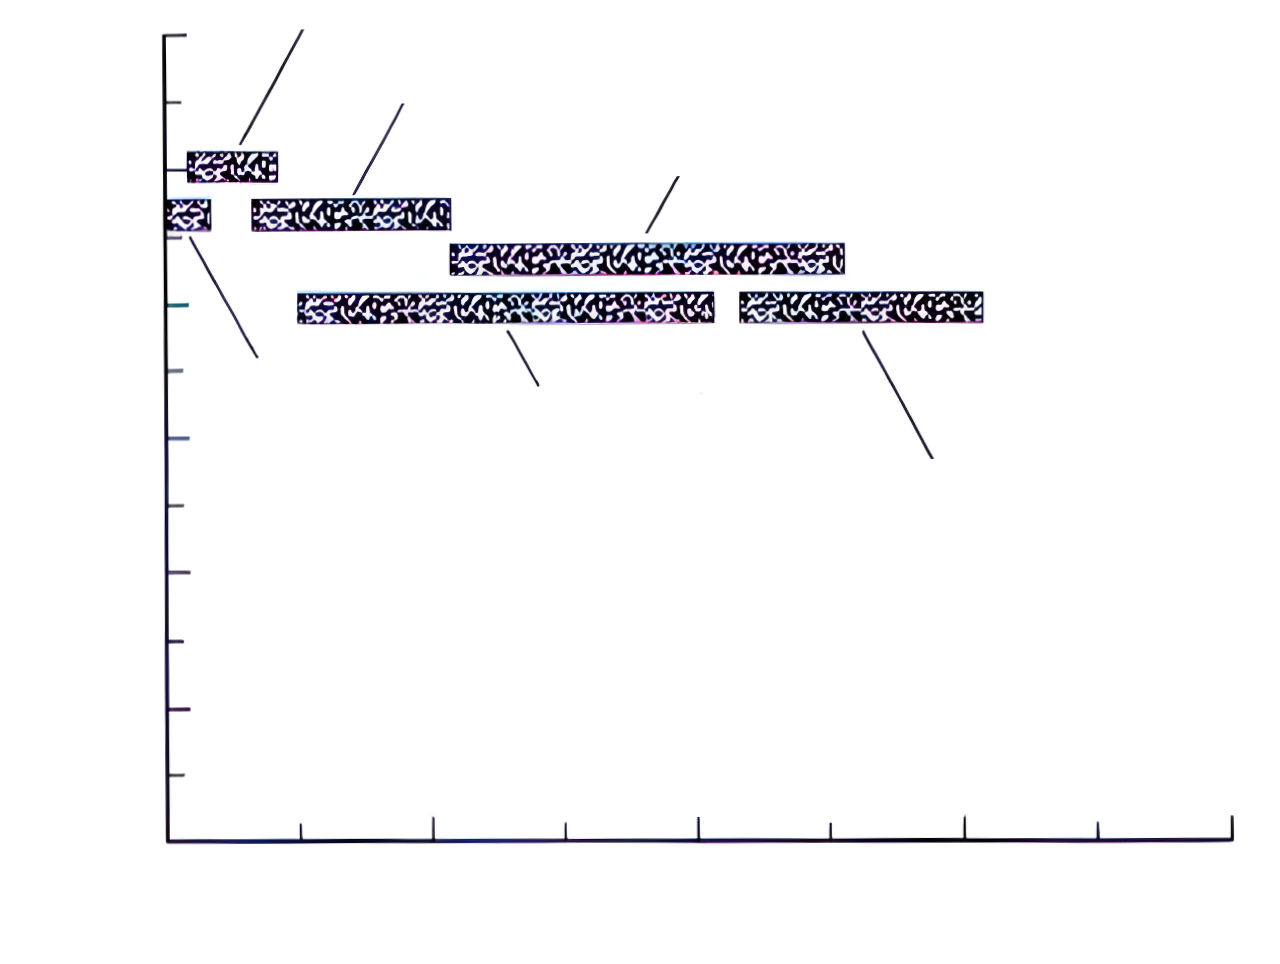
\includegraphics[width=0.68\textwidth]{figures/procesy_tap.png}};
\node[font=\small] at (2.6,-0.1) {Hydrokrakování};
\node[font=\small] at (0,0.5) {Hydrorafinace};
\node[font=\small,align=center] at (-2.3,0.5) {Katalytické\\krakování};
\node[font=\small] at (0.6,2.5) {Hydrovisbreaking};
\node[font=\small] at (-1.5,3) {Visbreaking};
\node[font=\small] at (-2.2,3.6) {Koksování};

\node[font=\small] at (-3.52,-3) {0};
\node[font=\small] at (-1.54,-3) {10};
\node[font=\small] at (0.44,-3) {20};
\node[font=\small] at (2.42,-3) {30};
\node[font=\small] at (4.4,-3) {40};
\node[font=\small] at (0.44,-3.48) {Tlak v reaktoru [MPa]};

\node[font=\small] at (-3.8,-2.67) {0};
\node[font=\small] at (-3.97,-1.7) {100};
\node[font=\small] at (-3.97,-0.71) {200};
\node[font=\small] at (-3.97,0.3) {300};
\node[font=\small] at (-3.97,1.29) {400};
\node[font=\small] at (-3.97,2.3) {500};
\node[font=\small] at (-3.97,3.3) {600};
\node[font=\small,rotate=90] at (-4.6,0.6) {Reakční teplota [$\mathrm{^{\circ}C}$]};
\end{tikzpicture}